%MIT OpenCourseWare: https://ocw.mit.edu
%RES.18-011 Algebra I Student Notes, Fall 2021
%License: Creative Commons BY-NC-SA 
%For information about citing these materials or our Terms of Use, visit: https://ocw.mit.edu/terms.

\section{Discrete Groups}
\subsection{Review}
Last time, we looked at discrete\footnote{The translations and rotations that cannot be arbitrarily small}  subgroups $G \leq M_2.$ Then, we looked at a projection $\pi$:
\begin{align*}
    \ker(\pi) &= (\RR^2, +) \subset M_2 \xrightarrow[]{\pi} O_2, \\
    t_b \circ A &\mapsto A;
\end{align*}
essentially, it gets rid of the translation part of an isometry. %Where $L$, the group of translations in $G,$ which is the symmetry group of $G,$, with the restriction of $\pi$ to $G,$ we get 

We can restrict $\pi$ to $G$ to get a mapping 
\[
G \xrightarrow[]{\pi|_G} O_2,
\]
and we call the kernel, 
\[
L \coloneqq \ker(\pi|_G),
\]

and it consists of all the translations in $G.$



%\[
%L \subset G \xrightarrow[]{\pi|_G} \overline{G} \coloneqq \pi(G),
%\]

The image of $G$ in $O_2$, denoted $\overline{G} \coloneqq \pi(G),$ is called the \emph{point group} of $G.$ For some element $g \in G,$ its image $\overline{g} \coloneqq \pi(g) \in \overline{G}$ only "remembers" the angle of rotation or the slope of the reflection line.

If $\overline{G}$ is discrete, it is either $C_n$ or $D_n,$ which we proved earlier.


If $L \subseteq \RR^2$ is discrete, then we obtained three possible cases. 
\begin{enumerate}[label = (\roman*)]
    \item $L = \{0\}$;
        \begin{center}
    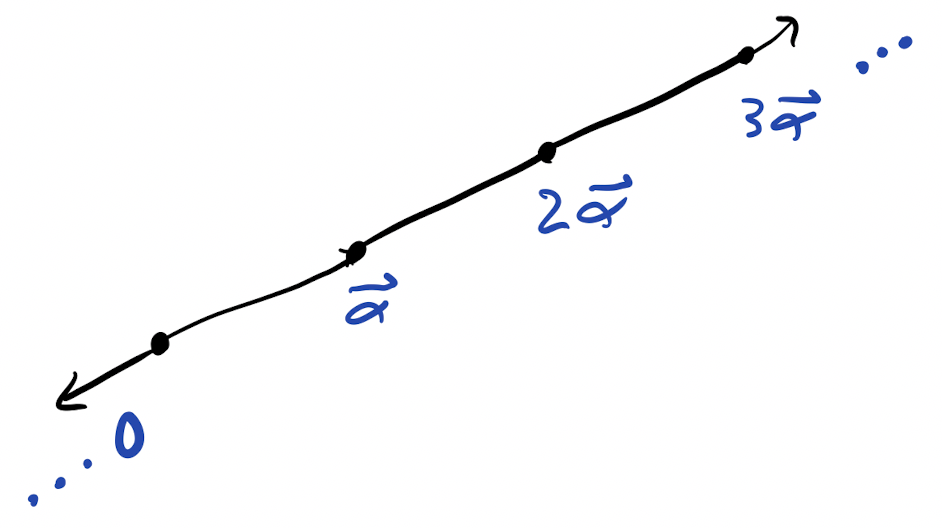
\includegraphics[width=6cm]{Lecture Files and Images/lec16-line.png}
\end{center}
    \item $L = \ZZ \alpha$ where $\alpha \neq 0;$
    \begin{center}
    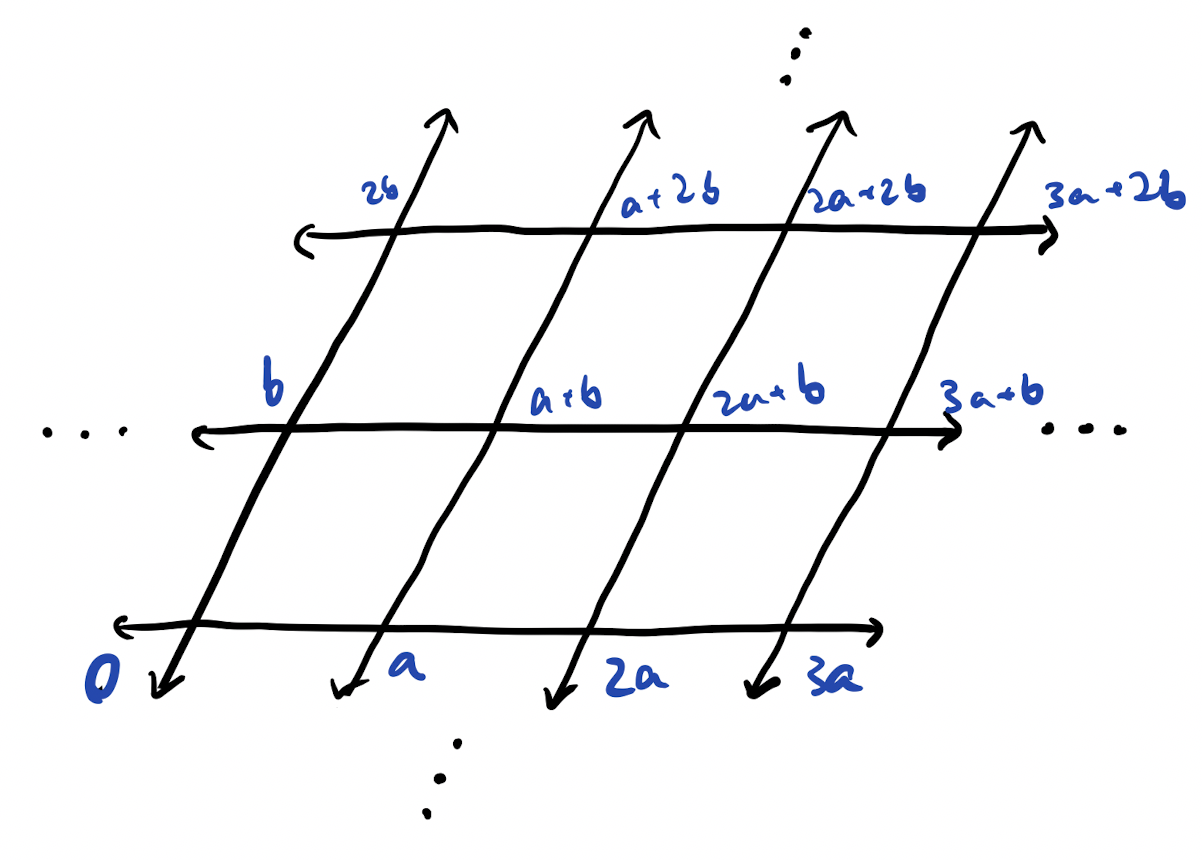
\includegraphics[width=6cm]{Lecture Files and Images/lec15-lattice.png}
\end{center}

    \item $L = \ZZ\alpha + \ZZ\beta$, where $\alpha, \beta$ are linearly independent.\footnote{When you look at two vectors and everything you generate from them, it's called a lattice.}%edit this 
    

\end{enumerate}

\subsection{Examples for \texorpdfstring{$L$}{L} and \texorpdfstring{$\overline{G}$}{G}}\label{examples for l and g}

For a given plane figure, it is actually not difficult to see what $L$ and $\overline{G}$ are! For the translation subgroup $L$, since it must either be the identity translation, $\ZZ\alpha$, or a lattice, it is possible to simply eyeball which translations preserve the figure. Let's consider the following plane figures. Later in this lecture, we will discuss the possibilities for $\overline{G}$; it consists of the (untranslated) rotations and reflections preserving a figure.




\begin{center}
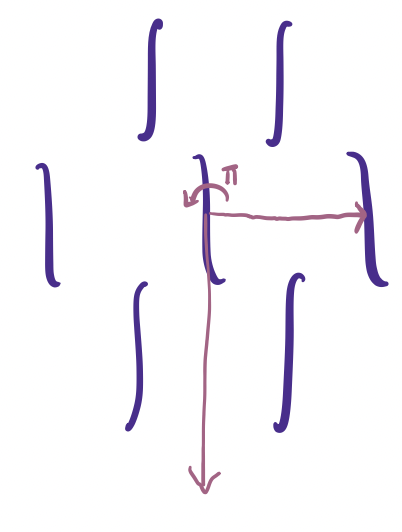
\includegraphics[width=4cm]{Lecture Files and Images/lec16-integrals.png}
\end{center}

\begin{example}[A]\label{example a}
For this first figure, say figure A, the translation subgroup $L$ is a rectangular lattice generated by two translation vectors, to the right and upward. Also, $\overline{G}$ is $D_2,$ since it contains a reflection as well as rotation by $\pi.$ 

\end{example}


\begin{center}
    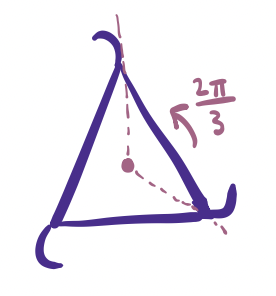
\includegraphics[width=3cm]{Lecture Files and Images/lec16-weirdtriangle.png}
\end{center}


\begin{example}[B]\label{example b}
For figure B, the translation subgroup is trivial, consisting of $0.$ Also, $\overline{G}$ is $C_3,$ since there cannot be any reflections but rotation by $2\pi/3$ or $4\pi/3$ around the center both preserve the figure.

\end{example}


\begin{center}
    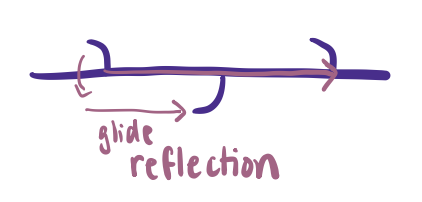
\includegraphics[width=5cm]{Lecture Files and Images/lec16-glide.png}
\end{center}

\begin{example}[C]\label{example c}
For figure C, the translation subgroup is generated by one vector, so $L = \ZZ\alpha$ where $\alpha = (1, 0)$. Also, $\overline{G}$ is $D_1,$ since there is a reflection (corresponding to a glide reflection in $G$) and no rotations possible. 
\end{example}


\begin{center}
    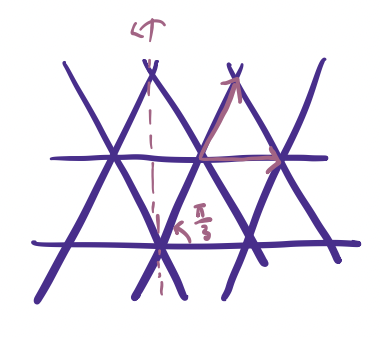
\includegraphics[width=5cm]{Lecture Files and Images/lec16-latticetriangle.png}
\end{center}
\begin{example}[D]\label{example d}
For figure D, the translation subgroup is a triangular lattice generated by two vectors at an angle of $\pi/3$ to each other.\footnote{Or two vectors at an angle of $2\pi/3$.} The point group is $\overline{G} = D_6,$ since rotation at a lattice point by any multiple of $\pi/3$ preserves the figure, as well as reflection. 

\end{example}

%write down 4:06

\subsection{Crystallographic Restriction}
Now that we have decomposed studying $G$ into studying groups we understand better, $L$, a subgroup of translations, and $\overline{G} \subseteq,$ the point group, we can actually constrain $G$ further! 

Recall that 
\begin{itemize}
    \item The translation subgroup $L \subseteq (\RR^2, +)$\footnote{The translation subgroup $L$ is sometimes written ambiguously in one of two equivalent ways; an element of $L$ can either be the translation $t_{\vec{b}} \in L$ considered as an element in $G,$ or simply the vector $\vec{b} \in L$ considered as an element in $\RR^2.$ So $L$ could be considered either as a subgroup of $G$ or of $\RR^2.$} must be one of three possibilities, which we get from studying discrete subgroups of $\RR^2$; %check if footnote makes sense LOL
    \item  $\overline{G}$ must be $C_n$ or $D_n,$ which we get from studying discrete subgroups of $O_2.$
\end{itemize}
 Now that we understand the components $L$ and $\overline{G}$ separately, we want to use this knowledge to understand $G$ better. %?? 11:17

\begin{qq}
How do $L$ and $\overline{G}$ interact with each other?
\end{qq}

\begin{example}
Consider our earlier example \ref{example d}. In this case, any element of the point group $D_6$ preserved the triangular lattice.
\end{example}

In fact, $\overline{G}$ acts on $L$ for any discrete group $G \subseteq M_2$; this is a very strong constraint on how $\overline{G}$ and $L$ interact.

\begin{theorem}\label{point group acts on l}
For the point group $\overline{G}\leq O_2$ of some discrete subgroup $G$ of $M_2,$ and the translation subgroup $L \subset \RR^2,$ the group $\overline{G}$ must map $L$ to itself. 

For any element $A \in \overline{G}$ and $b \in L,$ the image of $b$ under the action of $A$ is
\[
b \mapsto Ab \in L.
\]



%for any element of the point group $A \in \overline{G},$ and any element of the translation subgroup $b \in L,$ the element $A$ takes $b \mapsto Ab $ \mapsto Ab \in L.$
\end{theorem}

We already know that $O_2$ and thus $\overline{G}$ acts on the plane $\RR^2$ and therefore $L.$ The surprising part is that under the action of any element of $\overline{G}$, an element of $L$ is actually mapped to another element in $L$!


\begin{proof}
Since $A \in \overline{G},$ it is the image of an element of $G,$ say $t_{\vec{c}} \circ A \in G$ for some $\vec{c} \in \RR^2.$ Then, $\vec{b} \in L,$ so $t_{\vec{b}} \in G$. The key observation in this proof is that $L = \ker(\pi|_G)$ is the kernel of a homomorphism! Thus, the subgroup $L \nsub G$ is actually normal, so conjugating an element of $L$ by anything in $G$ stays in $L.$

Then for $t_{\vec{b}} \in L,$
\[
(t_{\vec{c}} \circ A) \cdot t_{\vec{b}} \cdot (t_{\vec{c}} \circ A)^{-1} \in L
\]
also. As isometries in $M_2,$ we know how to manipulate these products, and so expanding out this expression gives us 
\begin{align*}
    t_{\vec{c}} \cdot A \cdot t_{\vec{b}} \cdot A^{-1} \cdot t_{\vec{c}}^{-1} &= t_{\vec{c}} t_{A\vec{b}} \cdot A \cdot A^{-1} \cdot t_{-\vec{c}} \\
    &= t_{\vec{c}} t_{A\vec{b}} t_{-\vec{c}} \\
    &= t_{A\vec{b}} \in L.
\end{align*}

Thus, conjugating $t_{\vec{b}} \in L$ by $t_{\vec{c}} \circ A$ gives $t_{A\vec{b}} \in L.$ Using the identification of $L$ with $\RR^2,$ $A \vec{b} \in L \subset \RR^2$, and so every $A \in \overline{G}$ takes vectors $\vec{b}$ in $L$ to other vectors in $L,$ preserving the translation subgroup.
\end{proof}

\begin{question}%[Student Question]

We're studying discrete groups, which are groups with the requirement that the translations or rotations can't be arbitrarily small. Are we also requiring that they have to be groups preserving a given diagram, or can they be any discrete groups of isometries? 


%So with these discrete groups, we have a requirement that they can't be arbitrarily small but are we also saying that they can't be just any isometries they have to preserve the diagrams? 

\end{question}
\begin{ans}
Earlier on in this lecture, we saw some \textbf{examples} of discrete groups $G$ that came from the symmetry groups of certain diagrams, but what we are actually doing is simply looking at groups $G$ with the condition that the rotations and translations must be arbitarily small\footnote{These are called discrete groups}, and classifying them; mathematically, there is no requirement that they come from pictures. 

However, the way that these discrete groups actually show up and the way that we find them is by drawing these kinds of pictures; this is one of the main reasons why we care about them! In fact, for every discrete subgroup $G \subseteq M_2,$ there \emph{will be} some picture that produces the group $G$ as its symmetry group. The pictures in this lecture are mainly so that there are concrete examples to look at and think about. 

In Section \ref{examples for l and g}, each of the examples has a symmetry group $G$ consisting of the isometries of the plane sending the picture to itself.\footnote{Not each point individually is sent to itself; the picture as a whole is sent to an identical copy of itself.} For example, in Example \ref{example b}, rotation by 120 degrees preserves the "triangle," while 5 degrees does not, so $\rho_{2\pi/3} \in G,$ whereas $\rho_{\pi/36} \notin G.$ 

%what we are actually doing is taking some group $G$ and the rotations and translations can't be arbitrarily small. but they come from these pictures! IN FACT, for every $G$, there is some picture where $G$ is the symmetry group of this picture. 

\end{ans}

Theorem \ref{point group acts on l} states that the point group $\overline{G}$, which is a different group from $G,$ actually preserves $L \subseteq \RR^2,$ the translation group. 

In Example \ref{example d}, $L$ is generated by 
\[
\ZZ(1, 0)^t + \ZZ(1/2, 3/2)^t,
\]
the two sides of an equilateral triangle, and the point group is $D_6.$ Any element of $D_6$ will send an element of $L$ to a different element in $L.$

In fact, when $L$ is a lattice, preservation by some point group $\overline{G}$ is a strong constraint on the possible angles that show up in the lattice; only certain angles are allowed. Given $\overline{G},$ most lattices are not preserved by every element. Thus, the theorem constrains $\overline{G}$ and $L$ together --- not on each of them separately, but on how they interact. 

The groups that show up this way are often called crystallographic groups. \footnote{Especially when $L$ is a lattice, and there are two different directions to translate.} They are well-studied; in fact, there are only finitely many.

%question: is it the point group crystallographic? or the group G?

\begin{theorem}[Crystallographic Restriction]\footnote{The theorem name comes from the fact that it restricts the possible crystallographic groups.}
Let $L \neq \{0\}.$ Then $\overline{G} = C_n$ or $D_n$, where $n = 1, 2, 3, 4,$ or $6.$
\end{theorem}

%So before, it looked like we had lots of possibilities even before the discreteness condition, but since they have to interact with each other, it really narrows it down. Only certain choices of $L$ are allowed for a given $n.$

Although we could imagine that there are lots of possibilities for $\overline{G}$ and $L,$ the fact that $\overline{G}$ preserves $L$ constrains the possible point groups to finitely many, and there are also only certain choices of $L$ allowed for a given $n.$

%question: how many G are there total? is this true in higher dimensions?

\begin{proof}
The group $\overline{G}$ is a discrete subgroup of $O_2,$ and so it is $C_n$ or $D_n$ for some integer $n.$

Since $L$ is discrete, there is a (non-unique) shortest nonzero vector $\alpha \neq 0$. Consider a rotation $\rho = \rho_\theta \in G.$ The result of rotating $\alpha$ by $\theta$ is another vector in $L$, and since rotations are length-preserving, $\rho_{\theta} \alpha$ is also a vector of shortest length. Since both vectors are in $L,$  $\rho\alpha - \alpha$ is also in $L.$\footnote{Since $L$ is a subgroup, it is closed under addition/subtraction.} If $\theta$ is too small, $\rho\alpha - \alpha$ will have a shorter length, and there will be a contradiction. 

In particular, if $\theta < 2\pi/6,$ $\rho\alpha - \alpha$ is shorter than $\alpha$, so $\theta \geq 2\pi/6.$ Since $C_n$ and $D_n$ contain $\rho_{2\pi/n},$ it must be the case that $n \leq 6.$ 
\begin{center}
    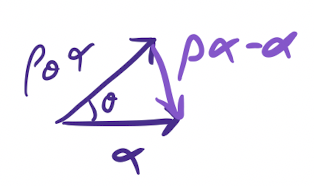
\includegraphics[width=4cm]{Lecture Files and Images/lec16-thetatriangle2.png}
\end{center}

A similar argument holds to rule out $n = 5.$ The vector $\alpha + \rho_{4\pi/5} \alpha$ will be shorter than any $\alpha$, which is also a contradiction.\footnote{This question is equivalent to the feasibility of tiling the plane with a regular pentagon, and in fact that is not possible!}%31:05

\begin{center}
    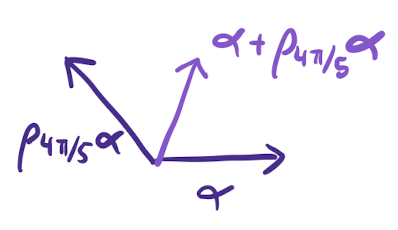
\includegraphics[width=4cm]{Lecture Files and Images/lec16-nis52.png}
\end{center}

So $n = 1, 2, 3, 4,$ or 6.  
\end{proof}
Actually, for $C_n$ or $D_n$ where $n = 1, 2, 3, 4$, or 6, it is possible to constrain the translation subgroups $L$ that can simultaneously show up.

For instance, when $L$ is a lattice,\footnote{When $L$ is a lattice, it is two-dimensional, and it is $\ZZ\vec{a} + \ZZ\vec{b}$ for generating vectors $\vec{a}$ and $\vec{b}.$ It is also possible for $L$ to be $\ZZ\vec{a}$, which is one-dimensional.} there are only 17 possible symmetry groups $G$ that can occur. When $L$ is 0, $\overline{G}$ can be $C_n$ or $D_n$ for any arbitrary $n$, but allowing nontrivial translations constrains $\overline{G}$ significantly.

\begin{question}%[Student Question]
How much does constraining $\overline{G}$ and $L$ constrain the actual symmetry group $G$ itself?
\end{question}

\begin{ans}
Finding $G$ from $\overline{G}$ and $L$ is precisely the same as figuring out the 17 plane symmetry groups,\footnote{These are called wallpaper groups, since wallpapers are 2-dimensional patterns that usually have nontrivial symmetry groups.} and is precisely the last step! We will do one example now.
\end{ans}

Let's consider a specific group $\overline{G}$ and try to figure out what the actual symmetry group $G$ can be!

\begin{example}[$C_4$]
Suppose $\overline{G} = C_4.$\footnote{Rotations by 90 degrees, but no reflections.} Then $L \subset G \xrightarrow[]{\pi|_G} C_4,$ and the index $[G: L] = 4.$\footnote{The index $[G: \ker(\pi|_G)] = [G:L]$ is equal to the size of the image under $\pi|_G$, which is $\overline{G} = C_4.$} 

Also, $\overline{\rho} = \rho_{\pi/2} \in \overline{G}$ is a generator of $\overline{G}.$ Where $\alpha$ is some shortest-length vector in $L,$ it's possible to show\footnote{There is a more involved argument there, but it is not super relevant here.} that $\rho\alpha$ and $\alpha$ do generate $L.$ Thus,
\[
L = \ZZ\alpha + \ZZ(\rho\alpha),
\]
a square lattice.

Also, there exists some rotation $\rho \in G$ giving $\pi(\rho) = \overline{\rho.}$ Then $\rho$ is in fact a rotation by $\pi/2$ around some other point, which we will call the origin.\footnote{In the discussion of the four kinds of isometries in $M_2,$ the elements which were mapped to rotations were in fact rotations around some point.} The group $G$ contains $L$, of index 4, as well as some rotation by $\pi/2,$ $\rho.$\footnote{The rotation $\rho$ is $\overline{\rho},$ lifted to be in $G,$ and it is an element of $G$ not in $L$ which generates the quotient, $C_4.$}

\begin{center}
    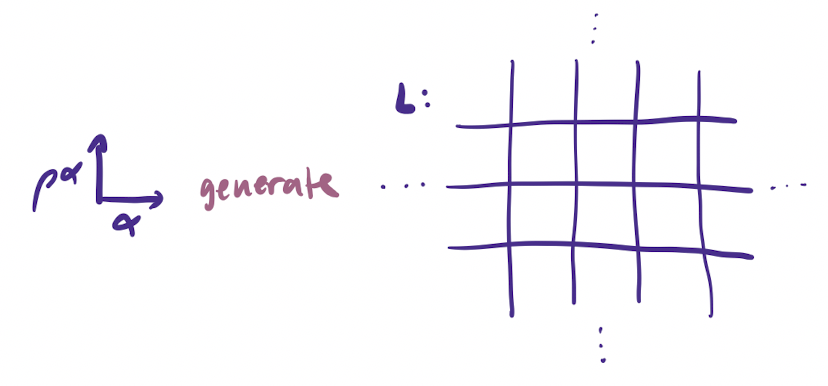
\includegraphics[width=5cm]{Lecture Files and Images/lec16-lattis.png}
\end{center}

Thus, $G$ is "generated" by $L$ and $\rho,$ and must consist of everything of the form 
\[
G = \{t_v \circ \rho^i: \vec{v} \in L, i = 0, 1, 2, 3\}.
\]

Also, $\rho t_v = t_{\rho v} \circ \rho,$ so the group multiplication can be written down, and $G$ is completely determined by knowing that $\overline{G}$ was $C_4$; this is 1 out of the 17 wallpaper groups!
\end{example}

\begin{question}
Can you explain where $\rho$ came from? Why is it a rotation? 
\end{question}

\begin{ans}
By definition, $\overline{G}$ is the image of $G$ under $\pi: M_2 \rightarrow O_2$ taking $t_b \circ A \mapsto A.$ Then there are four possibilities for elements in $M_2$: translation, rotations, reflections, and glide reflections. The first two are orientation-preserving, and the last two are orientation-reversing. Reflections and glide reflections map to reflections in $O_2$\footnote{Reflections across lines through the origin} under $\pi,$ translations will map to the identity, and rotations will map to rotations (around the origin). So $\rho$ has an image of $\overline{\rho},$ which is a rotation, and thus $\rho$ is a rotation around some point.
\end{ans}

If $\overline{\rho},$ the element in $\overline{G},$ were a reflection instead of a rotation, the preimage in $G$ could have been either a reflection or a glide reflection, so when the point group $\overline{G} = D_n$, one of the dihedral groups, instead of $C_n,$ the analysis is more subtle. In fact, there might not be any reflections in $G$ at all. (In Example \ref{example c}, there were no reflections, only glide reflections.) 

%A reflection $\overline{r} \in \overline{G}$ is $\pi(r)$ for $r \in G,$ where $r$ could be either a reflection or a glide reflection.

\begin{example}

If $\overline{r} = \pi(r)$ where $r$, then $\overline{r} = \pi(t_b \circ r_\ell),$ where $b$ is some zero\footnote{reflection} or nonzero\footnote{glide reflection} vector parallel to the line $\ell$. Does this mean there are uncountably many possibilities for $b$ and therefore $r?$ In fact, $b$ is constrained a bit more: $t_b r_\ell t_b r_\ell = t_{2b}$, so $2b \in L$. Thus, there are two possible situations: 
\begin{itemize}
    \item The vector is in the lattice: $b \in L$;
    \item The vector $b$ is halfway between two lattice points, as in Example \ref{example a}.
\end{itemize}
\end{example}

From these two examples, we see that given some $\overline{G}$, of which there are finitely many, and working through the information that is present, there aren't too many possibilities for $G$, and in fact there are finitely many --- 17 in total. 

\newpage